\documentclass[12pt,a4paper]{article}

% Margins.
\setlength{\oddsidemargin}{0in}
\setlength{\evensidemargin}{0in}
\setlength{\headheight}{12pt}
\setlength{\headsep}{42pt}
\setlength{\topmargin}{-54pt}
\setlength{\textwidth}{6.5in}
\setlength{\textheight}{10in}

\usepackage{amsmath}
\usepackage{float}
\usepackage{graphicx}
\usepackage[hyphens]{url}
\usepackage{hyperref}	% Clickable links to figures, references and urls.
\usepackage{enumerate}
\usepackage{datetime}

% Drawing.
\usepackage{pgf}
\usepackage{tikz}

% Listings for formatting code.
\usepackage{listings}
\usepackage{textcomp}
% General options.
\lstset{breaklines=true, basicstyle=\small\ttfamily, tabsize=4, numbers=left, stepnumber=1, frame=single, showstringspaces=false, upquote=true}
% C++ specific high-lighting. Comments are 50/50 shades of green/black and strings coloured with 60/40 red/black mixture.
\lstset{language=[ISO]C++, commentstyle=\color{green!50!black}, keywordstyle=\color{blue}, stringstyle=\color{red!60!black}}

%opening
\title{\vspace{-2cm}Programming for Engineers II\\Class 25\\Pointers and Arrays}
\author{Attique Dawood}
\date{March 29, 2013\\[0.2cm] Last Modified: \today, \currenttime}
\begin{document}
\maketitle
\section{Announcements}
\begin{itemize}
\item Quiz day. Quiz \# 6
\end{itemize}
\section{Revision}
\begin{itemize}
\item Dynamic memory allocation using pointer.
\item Need to overload copy constructor and assignment operator if copying pointers as data members.
\item Why copy constructor and assignment operator should have same code, default or otherwise? They're supposed to do the same thing. Need to make sure we're doing the same thing when any one of them is called.
\end{itemize}
\section{Dynamically Creating Objects}
\begin{itemize}
\item Just like ordinary variables, we can dynamically create objects.
\item A pointer to an object can be used to access data members with \verb|->| operator. Remember dot operator is used when we're using object variable.
\end{itemize}
\begin{lstlisting}[caption={Pointers to Objects}]
#include <iostream>
using namespace std;

class Complex
{
	public:
	float real, img;
};
int main()
{
	Complex* c;
	delete c; // What will this do? Crash! Don't try to de-allocate un-allocated pointers.

	c = new Complex; // Dynamic memory allocation.

	// Member access using arrow operator.
	c->real = 3; // Also, (*c).real
	c->img = 5;  // Also, (*c).img

	delete c; // De-allocation.

	// Array allocation.
	c = new Complex[10];

	for (int i=0; i<10; i++)
	{
		c[i].real = 3;
		c[i].img = 5;
	}
	delete[] c; // Release or de-allocate memory.

	return 0;
}
\end{lstlisting}
\section{Pointer Levels: Double Pointers}
This section is mostly taken from \cite{Ref:CPP-Double-Pointers}
\begin{itemize}
\item Treat everything, including pointers, as variables.
\item Keep normal variables at level 0.
\item Single pointers are at level 1.
\item Double pointers are at level 2 and so on.
\item Using variable name will access the value stored in the variable.
\item Dereferencing (a \verb|*| before variable name, e.g., \verb|*x|) takes you one level higher and gives you the respective value. Dereferencing a pointer always takes you to the variable which it `points' to.
\end{itemize}
\begin{figure}[H]
\centering
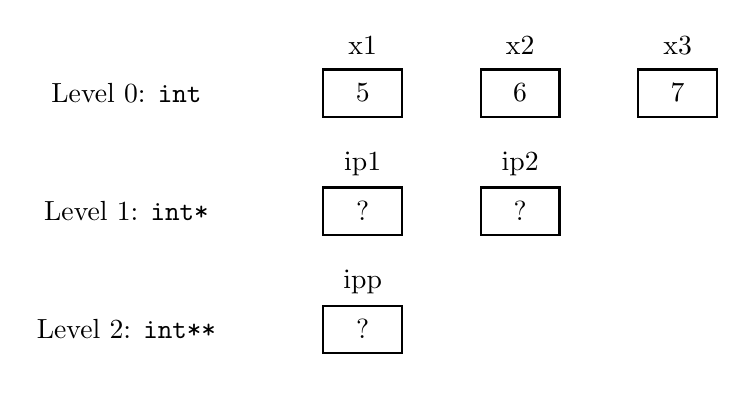
\begin{tikzpicture}
	% int
	\def\yd{0cm}
	\draw (0cm,\yd) node {Level 0: \texttt{int}};
	\foreach \x/\t/\val in {3cm/5/x1, 5cm/6/x2, 7cm/7/x3}
	{
		\draw[thick] (\x-0.5cm, \yd+0.3cm) rectangle (\x+0.5cm, \yd-0.3cm);
		\node[circle,minimum size=1cm] (\val) at (\x,\yd) {\t};
		\draw (\x,\yd+0.6cm) node {\val};
	}
	% int*
	\def\yd{-1.5cm}
	\draw (0cm,\yd) node {Level 1: \texttt{int*}};
	\foreach \x/\t/\val in {3cm/?/ip1, 5cm/?/ip2}
	{
		\draw[thick] (\x-0.5cm, \yd+0.3cm) rectangle (\x+0.5cm, \yd-0.3cm);
		\node[circle,minimum size=1cm] (\val) at (\x,\yd) {\t};
		\draw (\x,\yd+0.6cm) node {\val};
	}
	%\draw[thick,red,>=stealth,->,line width=2pt] (ip1) to [looseness=2,out=160,in=220] (x1);
	%\draw[thick,red,>=stealth,->,line width=2pt] (ip2) to [looseness=2,out=30,in=-60] (x2);
	%\draw[->,red] (ip1) edge[bend left] node (x1);
	%\draw [thick,red,->,>=stealth] plot [smooth] coordinates {(2.5cm,\yd) (2cm,\yd+1cm) (3cm,\yd+1.5cm)};
	% int**
	\def\yd{-3cm}
	\draw (0cm,\yd) node {Level 2: \texttt{int**}};
	\foreach \x/\t/\val in {3cm/?/ipp}
	{
		\draw[thick] (\x-0.5cm, \yd+0.3cm) rectangle (\x+0.5cm, \yd-0.3cm);
		\node[circle,minimum size=1cm] (\val) at (\x,\yd) {\t};
		\draw (\x,\yd+0.6cm) node {\val};
	}
	%\draw[thick,red,>=stealth,->,line width=2pt] (ipp) to [looseness=2,out=160,in=220] (ip2);
\end{tikzpicture}
\caption{Pointer Levels and Scenario after line 13}
\label{Pointer-Levels-and-Scenario-after-line-13}
\end{figure}
\begin{minipage}{5cm}
\begin{lstlisting}[caption={Pointer levels}]
#include <iostream>
using namespace std;

int main()
{
	int** ipp;

	int x1 = 5;
	int x2 = 6;
	int x3 = 7;

	int* ip1;
	int* ip2;

	ip1 = &x1;
	ip2 = &x2;
	ipp = &ip1;

	*ipp = ip2;
	*ipp = &x3;
	**ipp = -1;

	return 0;
}
\end{lstlisting}
\end{minipage}
\hspace*{1cm}
\begin{minipage}{10cm}
\begin{figure}[H]
\centering
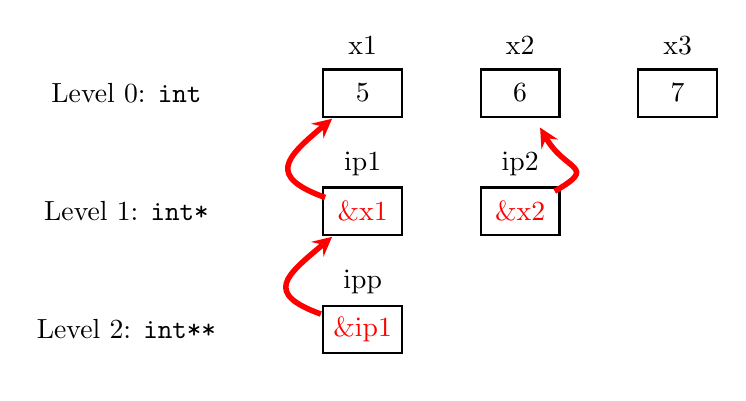
\begin{tikzpicture}
	% int
	\def\yd{0cm}
	\draw (0cm,\yd) node {Level 0: \texttt{int}};
	\foreach \x/\t/\val in {3cm/5/x1, 5cm/6/x2, 7cm/7/x3}
	{
		\draw[thick] (\x-0.5cm, \yd+0.3cm) rectangle (\x+0.5cm, \yd-0.3cm);
		\node[circle,minimum size=1cm] (\val) at (\x,\yd) {\t};
		\draw (\x,\yd+0.6cm) node {\val};
	}
	% int*
	\def\yd{-1.5cm}
	\draw (0cm,\yd) node {Level 1: \texttt{int*}};
	\foreach \x/\t/\val in {3cm/\textcolor{red}{\&x1}/ip1, 5cm/\textcolor{red}{\&x2}/ip2}
	{
		\draw[thick] (\x-0.5cm, \yd+0.3cm) rectangle (\x+0.5cm, \yd-0.3cm);
		\node[circle,minimum size=1cm] (\val) at (\x,\yd) {\t};
		\draw (\x,\yd+0.6cm) node {\val};
	}
	\draw[thick,red,>=stealth,->,line width=2pt] (ip1) to [looseness=2,out=160,in=220] (x1);
	\draw[thick,red,>=stealth,->,line width=2pt] (ip2) to [looseness=2,out=30,in=-60] (x2);
	%\draw[->,red] (ip1) edge[bend left] node (x1);
	%\draw [thick,red,->,>=stealth] plot [smooth] coordinates {(2.5cm,\yd) (2cm,\yd+1cm) (3cm,\yd+1.5cm)};
	% int**
	\def\yd{-3cm}
	\draw (0cm,\yd) node {Level 2: \texttt{int**}};
	\foreach \x/\t/\val in {3cm/\textcolor{red}{\&ip1}/ipp}
	{
		\draw[thick] (\x-0.5cm, \yd+0.3cm) rectangle (\x+0.5cm, \yd-0.3cm);
		\node[circle,minimum size=1cm] (\val) at (\x,\yd) {\t};
		\draw (\x,\yd+0.6cm) node {\val};
	}
	\draw[thick,red,>=stealth,->,line width=2pt] (ipp) to [looseness=2,out=160,in=220] (ip1);
\end{tikzpicture}
\caption{Scenario after line 17}
\label{Scenario-after-line-17}
\end{figure}
\begin{figure}[H]
\centering
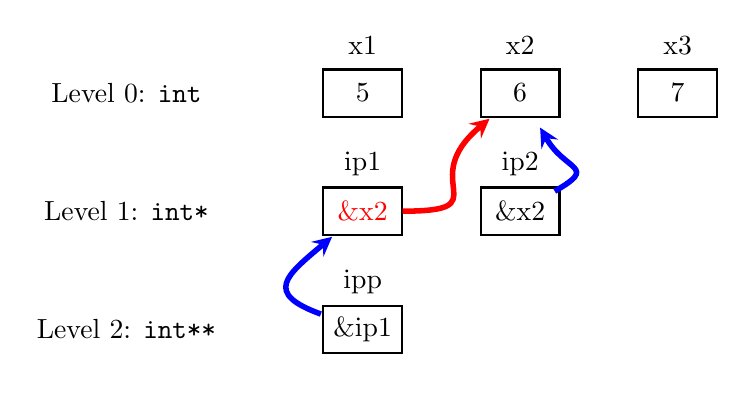
\begin{tikzpicture}
	% int
	\def\yd{0cm}
	\draw (0cm,\yd) node {Level 0: \texttt{int}};
	\foreach \x/\t/\val in {3cm/5/x1, 5cm/6/x2, 7cm/7/x3}
	{
		\draw[thick] (\x-0.5cm, \yd+0.3cm) rectangle (\x+0.5cm, \yd-0.3cm);
		\node[circle,minimum size=1cm] (\val) at (\x,\yd) {\t};
		\draw (\x,\yd+0.6cm) node {\val};
	}
	% int*
	\def\yd{-1.5cm}
	\draw (0cm,\yd) node {Level 1: \texttt{int*}};
	\foreach \x/\t/\val in {3cm/\textcolor{red}{\&x2}/ip1, 5cm/\&x2/ip2}
	{
		\draw[thick] (\x-0.5cm, \yd+0.3cm) rectangle (\x+0.5cm, \yd-0.3cm);
		\node[circle,minimum size=1cm] (\val) at (\x,\yd) {\t};
		\draw (\x,\yd+0.6cm) node {\val};
	}
	\draw[thick,red,>=stealth,->,line width=2pt] (ip1) to [looseness=2,out=0,in=220] (x2);
	\draw[thick,blue,>=stealth,->,line width=2pt] (ip2) to [looseness=2,out=30,in=-60] (x2);
	%\draw[->,red] (ip1) edge[bend left] node (x1);
	%\draw [thick,red,->,>=stealth] plot [smooth] coordinates {(2.5cm,\yd) (2cm,\yd+1cm) (3cm,\yd+1.5cm)};
	% int**
	\def\yd{-3cm}
	\draw (0cm,\yd) node {Level 2: \texttt{int**}};
	\foreach \x/\t/\val in {3cm/\&ip1/ipp}
	{
		\draw[thick] (\x-0.5cm, \yd+0.3cm) rectangle (\x+0.5cm, \yd-0.3cm);
		\node[circle,minimum size=1cm] (\val) at (\x,\yd) {\t};
		\draw (\x,\yd+0.6cm) node {\val};
	}
	\draw[thick,blue,>=stealth,->,line width=2pt] (ipp) to [looseness=2,out=160,in=220] (ip1);
\end{tikzpicture}
\caption{Scenario after line 19}
\label{Scenario-after-line-19}
\end{figure}
\end{minipage}
\begin{figure}[H]
\centering
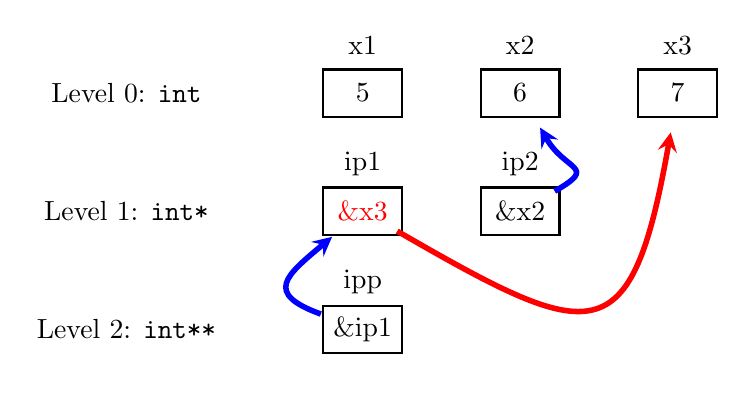
\begin{tikzpicture}
	% int
	\def\yd{0cm}
	\draw (0cm,\yd) node {Level 0: \texttt{int}};
	\foreach \x/\t/\val in {3cm/5/x1, 5cm/6/x2, 7cm/7/x3}
	{
		\draw[thick] (\x-0.5cm, \yd+0.3cm) rectangle (\x+0.5cm, \yd-0.3cm);
		\node[circle,minimum size=1cm] (\val) at (\x,\yd) {\t};
		\draw (\x,\yd+0.6cm) node {\val};
	}
	% int*
	\def\yd{-1.5cm}
	\draw (0cm,\yd) node {Level 1: \texttt{int*}};
	\foreach \x/\t/\val in {3cm/\textcolor{red}{\&x3}/ip1, 5cm/\&x2/ip2}
	{
		\draw[thick] (\x-0.5cm, \yd+0.3cm) rectangle (\x+0.5cm, \yd-0.3cm);
		\node[circle,minimum size=1cm] (\val) at (\x,\yd) {\t};
		\draw (\x,\yd+0.6cm) node {\val};
	}
	\draw[thick,red,>=stealth,->,line width=2pt] (ip1) to [looseness=2,out=-30,in=260] (x3);
	\draw[thick,blue,>=stealth,->,line width=2pt] (ip2) to [looseness=2,out=30,in=-60] (x2);
	%\draw[->,red] (ip1) edge[bend left] node (x1);
	%\draw [thick,red,->,>=stealth] plot [smooth] coordinates {(2.5cm,\yd) (2cm,\yd+1cm) (3cm,\yd+1.5cm)};
	% int**
	\def\yd{-3cm}
	\draw (0cm,\yd) node {Level 2: \texttt{int**}};
	\foreach \x/\t/\val in {3cm/\&ip1/ipp}
	{
		\draw[thick] (\x-0.5cm, \yd+0.3cm) rectangle (\x+0.5cm, \yd-0.3cm);
		\node[circle,minimum size=1cm] (\val) at (\x,\yd) {\t};
		\draw (\x,\yd+0.6cm) node {\val};
	}
	\draw[thick,blue,>=stealth,->,line width=2pt] (ipp) to [looseness=2,out=160,in=220] (ip1);
\end{tikzpicture}
\caption{Scenario after line 20}
\label{Scenario-after-line-20}
\end{figure}
\begin{figure}[H]
\centering
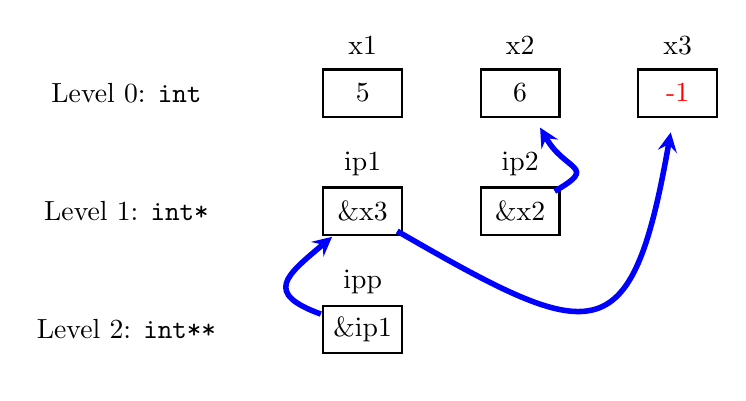
\begin{tikzpicture}
	% int
	\def\yd{0cm}
	\draw (0cm,\yd) node {Level 0: \texttt{int}};
	\foreach \x/\t/\val in {3cm/5/x1, 5cm/6/x2, 7cm/\textcolor{red}{-1}/x3}
	{
		\draw[thick] (\x-0.5cm, \yd+0.3cm) rectangle (\x+0.5cm, \yd-0.3cm);
		\node[circle,minimum size=1cm] (\val) at (\x,\yd) {\t};
		\draw (\x,\yd+0.6cm) node {\val};
	}
	% int*
	\def\yd{-1.5cm}
	\draw (0cm,\yd) node {Level 1: \texttt{int*}};
	\foreach \x/\t/\val in {3cm/\&x3/ip1, 5cm/\&x2/ip2}
	{
		\draw[thick] (\x-0.5cm, \yd+0.3cm) rectangle (\x+0.5cm, \yd-0.3cm);
		\node[circle,minimum size=1cm] (\val) at (\x,\yd) {\t};
		\draw (\x,\yd+0.6cm) node {\val};
	}
	\draw[thick,blue,>=stealth,->,line width=2pt] (ip1) to [looseness=2,out=-30,in=260] (x3);
	\draw[thick,blue,>=stealth,->,line width=2pt] (ip2) to [looseness=2,out=30,in=-60] (x2);
	%\draw[->,red] (ip1) edge[bend left] node (x1);
	%\draw [thick,red,->,>=stealth] plot [smooth] coordinates {(2.5cm,\yd) (2cm,\yd+1cm) (3cm,\yd+1.5cm)};
	% int**
	\def\yd{-3cm}
	\draw (0cm,\yd) node {Level 2: \texttt{int**}};
	\foreach \x/\t/\val in {3cm/\&ip1/ipp}
	{
		\draw[thick] (\x-0.5cm, \yd+0.3cm) rectangle (\x+0.5cm, \yd-0.3cm);
		\node[circle,minimum size=1cm] (\val) at (\x,\yd) {\t};
		\draw (\x,\yd+0.6cm) node {\val};
	}
	\draw[thick,blue,>=stealth,->,line width=2pt] (ipp) to [looseness=2,out=160,in=220] (ip1);
\end{tikzpicture}
\caption{Scenario after line 21}
\label{Scenario-after-line-21}
\end{figure}
\section{Pointers and Arrays}
The name of array is the pointer to its first element. A subscript besides array name can be translated in english as, ``access element located this much distance from start.'' Keep in mind that \verb|Array[i]| is the same as \verb|*(Array+i)| which means that you only need array pointer to access array elements using the subscript. Consider the following code
\begin{lstlisting}[caption={Arrays and Pointers}]
#include <iostream>
using namespace std;

int main()
{
	int Array[5] = {3,7,2,1,5};

	cout << Array << endl; // Prints the address of array.

	// Using subscript.
	cout << Array[0] << endl; // Print the value of element located a distance of 0 from start.
	cout << Array[3] << endl; // Print the value of element located a distance of 3 from start.
	cout << Array[5] << endl; // Print the value of element located a distance of 5 from start. ERROR! Out of bound.

	// Using Pointers.
	cout << *(Array+0) << endl; // Prints the value of first element which is 3.
	cout << *(Array+1) << endl; // Prints the value of second element which is 7.
	cout << *(Array+5) << endl; // Prints the value of sixth element which is out of bound. ERROR!

	return 0;
}
\end{lstlisting}
\begin{figure}[H]
\centering
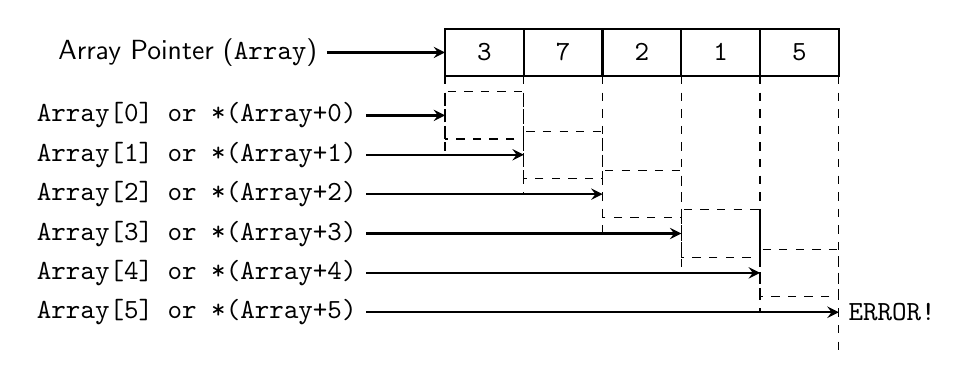
\begin{tikzpicture}
	% Writing 'Array'
	\coordinate [label=left:\textsf{Array Pointer (\texttt{Array})}] (Arraypointer) at (-1.5cm,0.3cm);
	\draw[thick, ->, >=stealth] (-1.5cm, 0.3cm) -- (0cm, 0.3cm);
	% Drawing boxes.
	\foreach \x in {0.0cm, 1.0cm, 2.0cm, 3.0cm, 4.0cm}
		\draw[thick] (\x, 0cm) rectangle (\x+1.0cm, 0.6cm);
	% Writing numbers in boxes. This is original array.
	\foreach \x/\y in {0.0cm/3, 1.0cm/7, 2.0cm/2, 3.0cm/1, 4.0cm/5}
		\draw (\x+0.5cm,0.3cm) node {\texttt{\y}};
	\def\XD{0cm}
	\def\YD{-0.5cm}
	% Drawing an arrow and pointer.
	\coordinate [label=left:\texttt{Array[0] or *(Array+0)}] (Array0) at (-1cm,\YD);
	\draw[thick, ->, >=stealth] (-1cm, \YD) -- (0cm+\XD, \YD);
	\draw[dashed] (\XD,0cm) -- (\XD,\YD-0.5cm);
	\draw[dashed] (\XD,\YD-0.3cm) rectangle (\XD+1cm,\YD+0.3cm);

	\def\XD{1cm}
	\def\YD{-1cm}
	% Drawing an arrow and pointer.
	\coordinate [label=left:\texttt{Array[1] or *(Array+1)}] (Array1) at (-1cm,\YD);
	\draw[thick, ->, >=stealth] (-1cm, \YD) -- (0cm+\XD, \YD);
	\draw[dashed] (\XD,0cm) -- (\XD,\YD-0.5cm);
	\draw[dashed] (\XD,\YD-0.3cm) rectangle (\XD+1cm,\YD+0.3cm);

	\def\XD{2cm}
	\def\YD{-1.5cm}
	% Drawing an arrow and pointer.
	\coordinate [label=left:\texttt{Array[2] or *(Array+2)}] (Array2) at (-1cm,\YD);
	\draw[thick, ->, >=stealth] (-1cm, \YD) -- (0cm+\XD, \YD);
	\draw[dashed] (\XD,0cm) -- (\XD,\YD-0.5cm);
	\draw[dashed] (\XD,\YD-0.3cm) rectangle (\XD+1cm,\YD+0.3cm);

	\def\XD{3cm}
	\def\YD{-2cm}
	% Drawing an arrow and pointer.
	\coordinate [label=left:\texttt{Array[3] or *(Array+3)}] (Array3) at (-1cm,\YD);
	\draw[thick, ->, >=stealth] (-1cm, \YD) -- (0cm+\XD, \YD);
	\draw[dashed] (\XD,0cm) -- (\XD,\YD-0.5cm);
	\draw[dashed] (\XD,\YD-0.3cm) rectangle (\XD+1cm,\YD+0.3cm);
	
	\def\XD{4cm}
	\def\YD{-2.5cm}
	% Drawing an arrow and pointer.
	\coordinate [label=left:\texttt{Array[4] or *(Array+4)}] (Array4) at (-1cm,\YD);
	\draw[thick, ->, >=stealth] (-1cm, \YD) -- (0cm+\XD, \YD);
	\draw[dashed] (\XD,0cm) -- (\XD,\YD-0.5cm);
	\draw[dashed] (\XD,\YD-0.3cm) rectangle (\XD+1cm,\YD+0.3cm);
	
	\def\XD{5cm}
	\def\YD{-3cm}
	% Drawing an arrow and pointer.
	\coordinate [label=left:\texttt{Array[5] or *(Array+5)}] (Array5) at (-1cm,\YD);
	\draw[thick, ->, >=stealth] (-1cm, \YD) -- (0cm+\XD, \YD);
	\draw[dashed] (\XD,0cm) -- (\XD,\YD-0.5cm);
	\coordinate [label=right:\texttt{ERROR!}] (Error) at (\XD,\YD);
\end{tikzpicture}
\caption{Using pointer to access array elements}
\label{Array-pointer-element-access}
\end{figure}
\begin{figure}[H]
\centering
\begin{tikzpicture}
	% int
	\def\yd{0cm}
	\draw (0cm,\yd) node {Level 0: \texttt{int}};
	\foreach \x/\t/\val in {3cm/3/Array[0], 4cm/7/, 5cm/2/, 6cm/1/, 7cm/5/}
	{
		\draw[thick] (\x-0.5cm, \yd+0.3cm) rectangle (\x+0.5cm, \yd-0.3cm);
		\node[circle,minimum size=1cm] (\val) at (\x,\yd) {\t};
		\draw (\x,\yd+0.6cm) node {\val};
	}
	% int*
	\def\yd{-1.5cm}
	\draw (0cm,\yd) node {Level 1: \texttt{int*}};
	\foreach \x/\t/\val in {3cm/\&Array[0]/Array}
	{
		\draw[thick] (\x-1cm, \yd+0.3cm) rectangle (\x+1cm, \yd-0.3cm);
		\node[] (\val) at (\x,\yd) {\t};
		\draw (\x,\yd+0.6cm) node {\val};
	}
	\draw[thick,red,>=stealth,->,line width=2pt] (ip1) to [looseness=2,out=240,in=200] (Array[0]);
	%\draw[thick,blue,>=stealth,->,line width=2pt] (ip2) to [looseness=2,out=30,in=-60] (x2);
	%\draw[->,red] (ip1) edge[bend left] node (x1);
	%\draw [thick,red,->,>=stealth] plot [smooth] coordinates {(2.5cm,\yd) (2cm,\yd+1cm) (3cm,\yd+1.5cm)};
\end{tikzpicture}
\caption{Accessing array using pointer}
\label{Accessing-Array-as-Pointer}
\end{figure}
\section{Dynamic 2D Array Using Double Pointer}
\begin{itemize}
\item An int* can be used to create a 1D array of ints.
\item Multiple int* 'ers can be used to create multiple 1D arrays.
\item Multiple 1D arrays form a 2D array.
\item An int** can be used to create a 1D array of int* 'ers.
\end{itemize}
\begin{figure}[H]
\centering
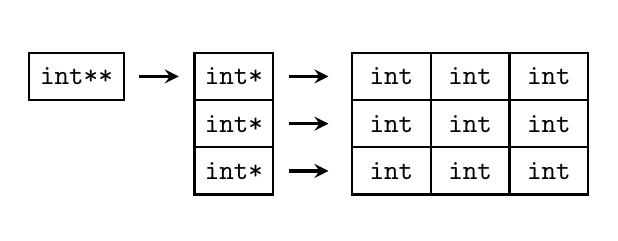
\begin{tikzpicture}
	\def\yd{0cm}
	\def\xd{0cm}
	% int**
	\draw[thick] (\xd-2.6cm, \yd+0.3cm) rectangle (\xd-1.4cm, \yd-0.3cm);
	\node[circle,minimum size=1cm] (intp) at (\xd-2cm,\yd) {\texttt{int**}};
	\draw[->,>=stealth,very thick] (\xd-1.2cm,\yd) -- (\xd-0.7cm,\yd);
	% int* array
	%\draw (0cm,\yd) node {Level 0: \texttt{int}};
	\foreach \y in {0cm, -0.6cm, -1.2cm}
	{
		\draw[thick] (\xd-0.5cm, \y+0.3cm) rectangle (\xd+0.5cm, \y-0.3cm);
		\node[circle,minimum size=1cm] (intp) at (\xd,\y) {\texttt{int*}};
		\draw[->,>=stealth,very thick] (\xd+0.7cm,\y) -- (\xd+1.2cm,\y);
		\foreach \x in {2cm, 3cm, 4cm}
		{
			\draw[thick] (\x-0.5cm, \y+0.3cm) rectangle (\x+0.5cm, \y-0.3cm);
			\node[circle,minimum size=1cm] (intp) at (\x,\y) {\texttt{int}};
		}
	}
\end{tikzpicture}
\caption{Dynamic 2D array concept}
\label{Dynamic-2D-array-concept}
\end{figure}
\begin{lstlisting}[caption={Dynamic 2D array}]
int main()
{
	int Rows = 3;
	int Cols = 3;
	// Pointer.
	int** Array2D;

	// Array of int* 'ers equal to number of rows.
	Array2D = new int*[Rows];
	// Each int* is used to allocate int array equal to number of columns.
	for (int i=0; i<Rows; i++)
	{
		Array2D[i] = new int[Cols];
	}

	// Accessing array elements.
	for (int i=0; i<Rows; i++)
	{
		for (int j=0; j<Cols; j++)
		{
			Array2D[i][j] = i*j;
		}
	}
	// Array2D[i][j] = *((*(Array2D+i))+j) = (*(Array2D+i))[j] = *(Array2D[i]+j)

	// De-allocation
	for (int i=0; i<Rows; i++)
	{
		delete[] Array2D[i];
	}
	delete[] Array2D;

	return 0;
}
\end{lstlisting}
%\nocite{*}
\bibliographystyle{plain}
\bibliography{OOPref}
\end{document}
